\section{Generalization-Oriented Parameter Setting}
\begin{figure}[t]
    \centering
    \begin{subfigure}[t]{0.32\linewidth}
        \centering
        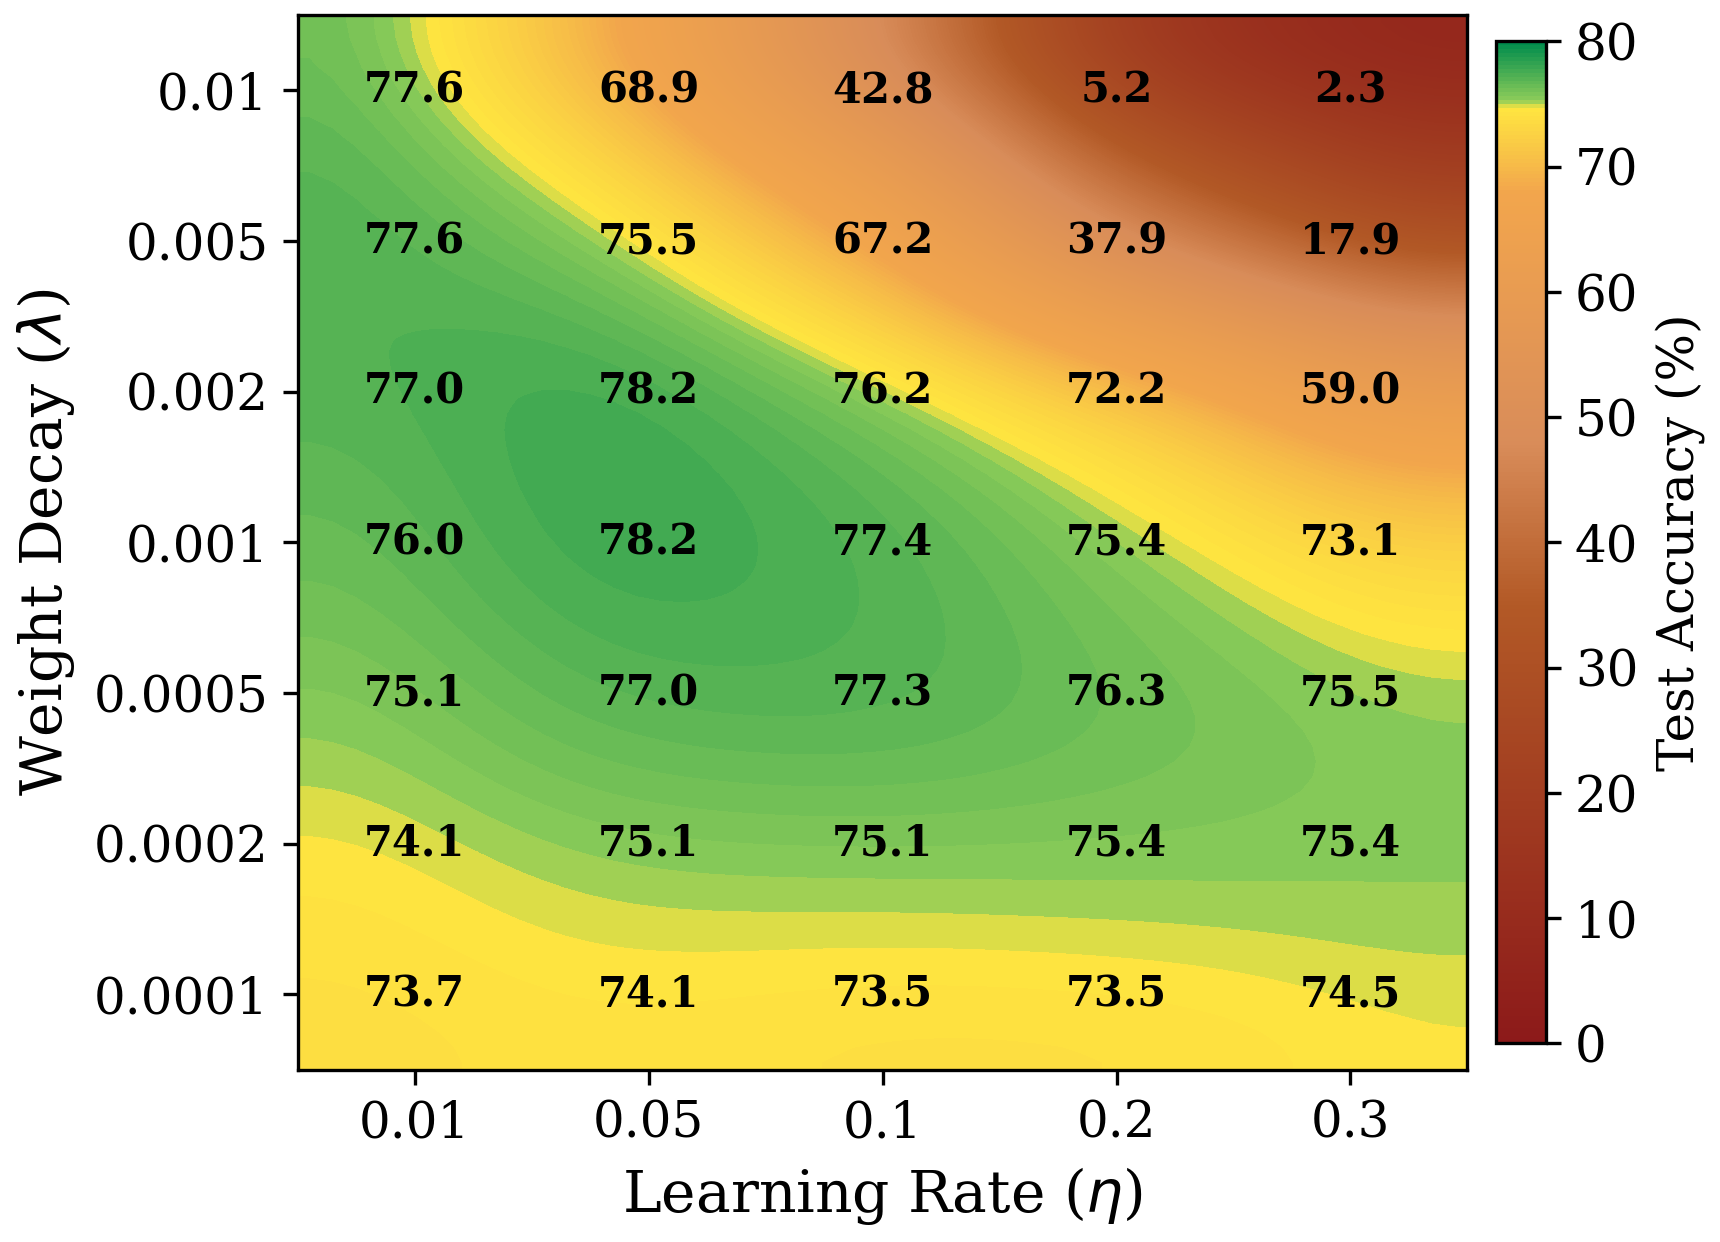
\includegraphics[width=\linewidth]{figures/exp2_heatmap_r18.png}
        \caption{$\eta$--$\lambda$ heatmap. The high-accuracy region forms a clear anti-diagonal band, consistent with the stability bound $\eta(1+\lambda)<2/L$.}
        \label{fig:WD and LR-heatmap}
    \end{subfigure}
    \hfill
    \begin{subfigure}[t]{0.32\linewidth}
        \centering
        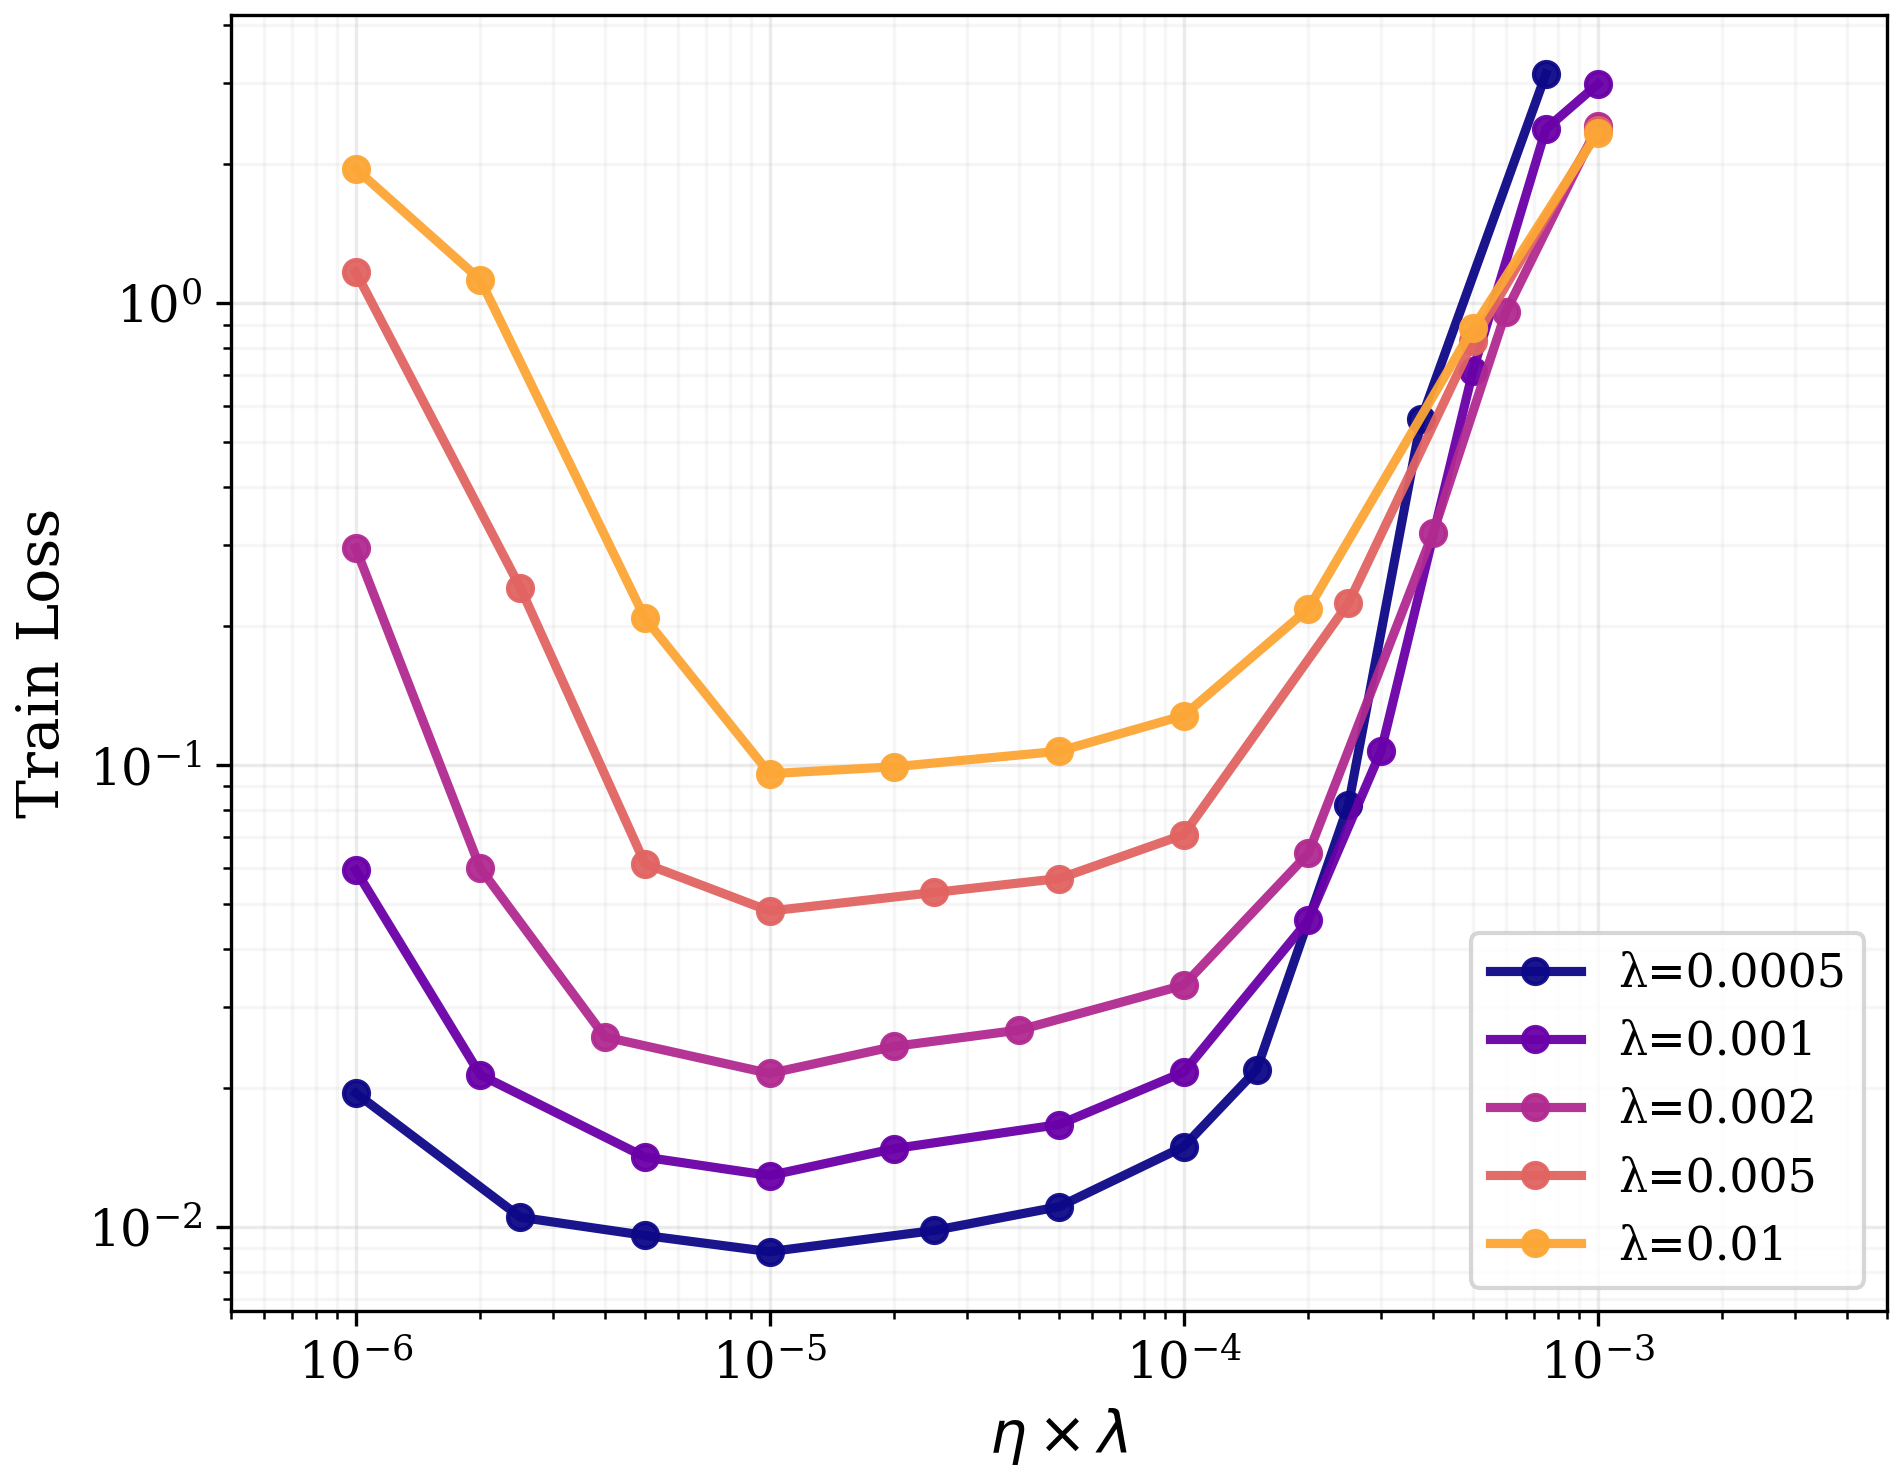
\includegraphics[width=\linewidth]{figures/exp2_train_curve.png}
        \caption{Train loss vs.\ joint product $\eta\times\lambda$ (each curve fixes one $\lambda$). Stars mark per-curve minima.}
        \label{fig:WD and LR-train}
    \end{subfigure}
    \hfill
    \begin{subfigure}[t]{0.32\linewidth}
        \centering
        
\includegraphics[width=\linewidth]{figures/exp2_eta_lambda_smooth.png}
        \caption{Best test accuracy vs.\ $\eta\times\lambda$. All fixed-$\lambda$ curves peak inside the same narrow band (dashed grey), directly verifying $\lambda\approx C/(\eta T)$.}
        \label{fig:WD and LR-smooth}
    \end{subfigure}
    \caption{Coupled effect of learning rate $\eta$ and weight decay $\lambda$. 
    (a) The full $\eta$--$\lambda$ heatmap; the optimal $\lambda^{*}$ decreases monotonically with $\eta$. 
    (b)~Train loss replotted against the joint product $\eta\times\lambda$: each fixed-$\lambda$ curve attains its minimum inside a common, narrow $\eta\times\lambda$ band. 
    (c)~Best test accuracy as a function of $\eta\times\lambda$: every curve peaks inside the same band, providing a quantitative confirmation of the inverse scaling law in Eq.~\eqref{coupling:lamda} that does not rely on diagonal heatmap reading.}
    \label{fig:WD and LR}
    \vspace{-0.8em} 
\end{figure}

\begin{tcolorbox}
\textbf{Q2:} Can we derive a quantitative scaling Law via uniform stability theory that precisely reveals the intrinsic coupling mechanism between $\lambda$, $\eta$, $B$, and other parameters?
\end{tcolorbox}

\citet{wang2025setadamwsweightdecay} model AdamW as an Exponential Moving Average (EMA). Through formal analogy, they derived an explicit relationship among $\lambda$, $\eta$, and $T$: $\lambda = \frac{1}{\eta T}$, implying an inverse proportionality between the learning rate and weight decay when the number of iterations $T$ is fixed. 

Building on the "Regularization Equivalence" hypothesis proposed in this work, we seek to quantify the interplay between hyperparameters through the lens of Uniform Stability. Instead of treating hyperparameters in isolation, we postulate that SGD-WD and SWA should satisfy comparable stability constraints to achieve identical generalization. This theoretical alignment allows us to derive the implicit coupling relationship, laying the mathematical foundation for the scaling laws proposed in this work.

\subsection{Coupling of $\lambda$ and $\eta$}
We first present the generalized bound for the SWA.

\begin{lemma}{\rm (\citet[Theorem 4.1]{pmlr-v235-wang24bl})}\label{thm:SWA}
Assume that the loss function $F(\theta;z)$ is convex, Lipschitz and $L$-smooth for all given $z\in\mathcal{Z}$ with sizes $n$. Suppose we run WA with step sizes $\eta \leq \frac{2}{L}$ for $T$ steps, where each step samples $z_i$ from $\mathcal{Z}$ without replacement. Then, WA has uniform stability of
\begin{equation}
  \epsilon_{gen} = \mathbb{E}\vert F(\bar{\theta}_T;z)-F(\bar{\theta}^{\prime}_T;z)\vert \leq \frac{\eta G^2 T}{n}.
 \end{equation}
\end{lemma}

\begin{remark}
Lemma \ref{thm:SWA} shows that under the assumption of convexity, the generalization bound of SWA is half that of SGD, implying a significant improvement in generalization performance. This is a well-established result, and its detailed proof can be found in \cite{pmlr-v235-wang24bl,hardt2016train,xiao2022stability}. 
\end{remark}

By bridging the generalization bounds of SGD-WD (Theorem \ref{thm:sgd-WD}) and SWA (Theorem \ref{thm:SWA}) under the Regularization Equivalence hypothesis, we equate their stability constraints to obtain the following scaling relationship:
\begin{equation}\label{coupling:lamda}
\lambda \approx \frac{C}{\eta T}, %\implies \lambda \eta T \approx \text{Constant} 
\end{equation}
where $C$ subsumes constant factors. It captures the dependency relationship between $\eta$ and $\lambda$ that must be followed to maintain system stability across varying training durations.

\begin{remark}
Eq.~\eqref{coupling:lamda} predicts that for a fixed iteration $T$, $\lambda$ must scale inversely with $\eta$. This theoretical derivation corroborates recent empirical findings in \cite{wang2025setadamwsweightdecay,bergsma2025powerlinesscalinglaws}. As visualized in the middle of Fig. \ref{fig:WD and LR}, our experimental data aligns well with this theoretical curve $1/x$, confirming that the heuristic alignment of stability bounds successfully captures the intrinsic coupling.
\end{remark}

\begin{remark}
Eq.~\eqref{coupling:lamda} suggests that $\eta$ and $\lambda$ play commensurate roles in the system. This implies that extreme concurrent configurations of these parameters will destabilize the training process. As demonstrated in the left and right of Figure \ref{fig:WD and LR}, the model attains optimal generalization only when the joint product of these hyperparameters (e.g., $\eta \cdot \lambda$) is maintained within an appropriate interval.
\end{remark}

 \subsection{Coupling of $\lambda$, $\eta$ and $B$}
To explicitly incorporate the batch size $B$, we rewrite the total iterations as $T = T_{epo} \cdot (n/B)$. Substituting this into Eq.~\eqref{coupling:lamda} yields the batch-dependent scaling law:
\begin{equation}\label{coupling:Batch}
\lambda \approx \frac{B}{\eta n T_{epo}}.
\end{equation}

\begin{figure*}[t]
    \centering
    
\includegraphics[width=\linewidth]{figures/batch.png}
    \caption{Coupling effects among hyperparameters at optimal performance after introducing batch size $B$. Top: For a fixed $\lambda$, the left and right subplots compare model performance across different $\eta$ with $B=32$ and $B=128$, respectively. Middle: Comparison of the optimal performance against the joint values of $\lambda\times\eta$ for $B=32$ (left) and $B=128$ (right). Bottom: For a fixed $\eta$, the left and right subplots compare model performance across different weight decay values $\lambda$ with $B=32$ and $B=128$, respectively.}
    \label{fig:batch}
    \vspace{-1em}  
\end{figure*}
 
\begin{remark}
Eq.~\eqref{coupling:Batch} reveals a fundamental compensation mechanism between explicit and implicit regularization. Small-batch training introduces significant gradient noise, acting as a strong implicit regularizer. As $B$ increases, this noise diminishes, creating a "regularization deficit." Consequently, to conserve total stability, the explicit weight decay $\lambda$ (and learning rate $\eta$) must be scaled up proportionally to compensate. This theoretical insight perfectly matches the empirical trends in Figure~\ref{fig:batch}, where increasing $B$ from 32 to 128 necessitates shifting the optimal $\lambda$ from $5\text{e-}4$ to $1\text{e-}3$.
\end{remark}

\textbf{Answer to Q2:} As shown in Eq. \ref{coupling:lamda} and \ref{coupling:Batch}, $\lambda$ acts as a counterweight to $\eta \cdot T$, requiring an inverse adjustment to maintain equilibrium, as validated by experience in Figure \ref{fig:WD and LR}. When Batch Size $B$ is introduced, it acts as a scaling factor: larger batches reduce implicit noise, necessitating a proportional increase in the joint magnitude of $\lambda$ and $\eta$ to preserve the stability, as shown in the Figure \ref{fig:batch} and Figure \ref{fig:LLM1} (the latter verified using LLM).


% \begin{remark}
% This scaling law offers actionable guidance for constrained scenarios. In resource-limited regimes (small $B$), one should reduce the joint product $\lambda \cdot \eta$ to prevent over-regularization (since noise is already high). Conversely, in throughput-prioritized regimes (large $B$), one can explore a larger $\lambda \cdot \eta$ product to accelerate convergence without sacrificing stability, consistent with the results in Figure \ref{fig:batch} (Middle).
% \end{remark}

% \begin{remark}
% Under practical constraints, such as limited computational resources where only small batch sizes are feasible, the proposed scaling law suggests selecting $\lambda\times\eta$ at lower values to ensure better test performance. In contrast, when computational resources are sufficient and efficiency is prioritized, a larger $\lambda\times\eta$ can be explored, which is consistent with the trend shown in the middle of Figure \ref{fig:batch}.
% \end{remark}

